\chapter{Creating analysis pipelines - Using Cellprofiler}
\section{Cellprofiler}
In the preceeding modules you got familiar with the concept of
analysis workflows and a selection of their possible components. In
this module you will learn to know cellprofiler another software tool
specialized in implementing and automating analysis pipelines.

\subsection{A simple pipeline}

\begin{taskbox}{Measure number and size of lysosomes per cell}



\begin{enumerate}
\item Start the Cellprofiler software and wait for the graphical user interface to appear. Shortly acknowledge
the resources advertised in the Welcome Screen and then close the Welcome Screen window.
Drag and drop the file \texttt{hela-cells.tif} from \texttt{data/mod2} into the drop-zone.

\item Proceed to the Metadata module. Select: \newline
\texttt{Extract Metadata}: \texttt{YES} \newline
\texttt{Metadata extraction method}: \texttt{Extract from image file headers}

Click \texttt{Update Metadata} button and then the \texttt{Update} above the metadata table (cf. Fig. \ref{fig:cpMetadata}).


	\begin{minipage}[t]{\linewidth}
		\begin{center}
		\adjustbox{valign=t}{%
		  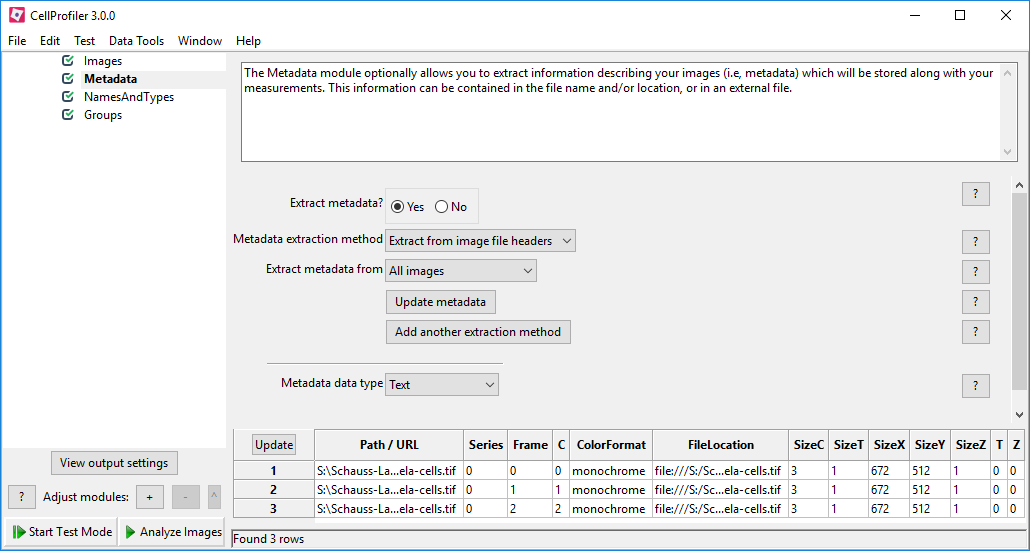
\includegraphics[width=0.70\textwidth]{mod4/figures/cpMetadata.png}
		  		}
		\medskip
		\captionof{figure}{Cellprofiler metadata module.}\label{fig:cpMetadata}
		\end{center}
	\end{minipage}


\item Now three data rows should be displayed. In case there is just one line, save your project \texttt{[File>Save
Project]}, then close the project and open it anew without closing Cellprofiler. Now repeat \texttt{Update
Metadata} and \texttt{Update}.

\item Proceed to the NamesAndTypes module. Select:\newline
\texttt{Assign a name to}: \texttt{Images matching rules}

\item In the dropdown menus below \texttt{Select the rule criteria…}, set \newline 
\texttt{Metadata – Does – Have C matching – 0}\newline
\texttt{Name to assign these images: LysosomesImage}.\newline
Press the \texttt{Duplicate this Image} button. In the new section change the value for \texttt{C} to \texttt{1} and assign
\texttt{MitochondriaImage} as name. Press \texttt{Duplicate this Image} again and in the new section change the value for
\texttt{C} to \texttt{2} and assign \texttt{NucleusImage} as name (cf. Fig. \ref{fig:cpNamesAndTypes}). Press the \texttt{Update} button above the image table.
	\begin{minipage}[t]{\linewidth}
		\begin{center}
		\adjustbox{valign=t}{%
		  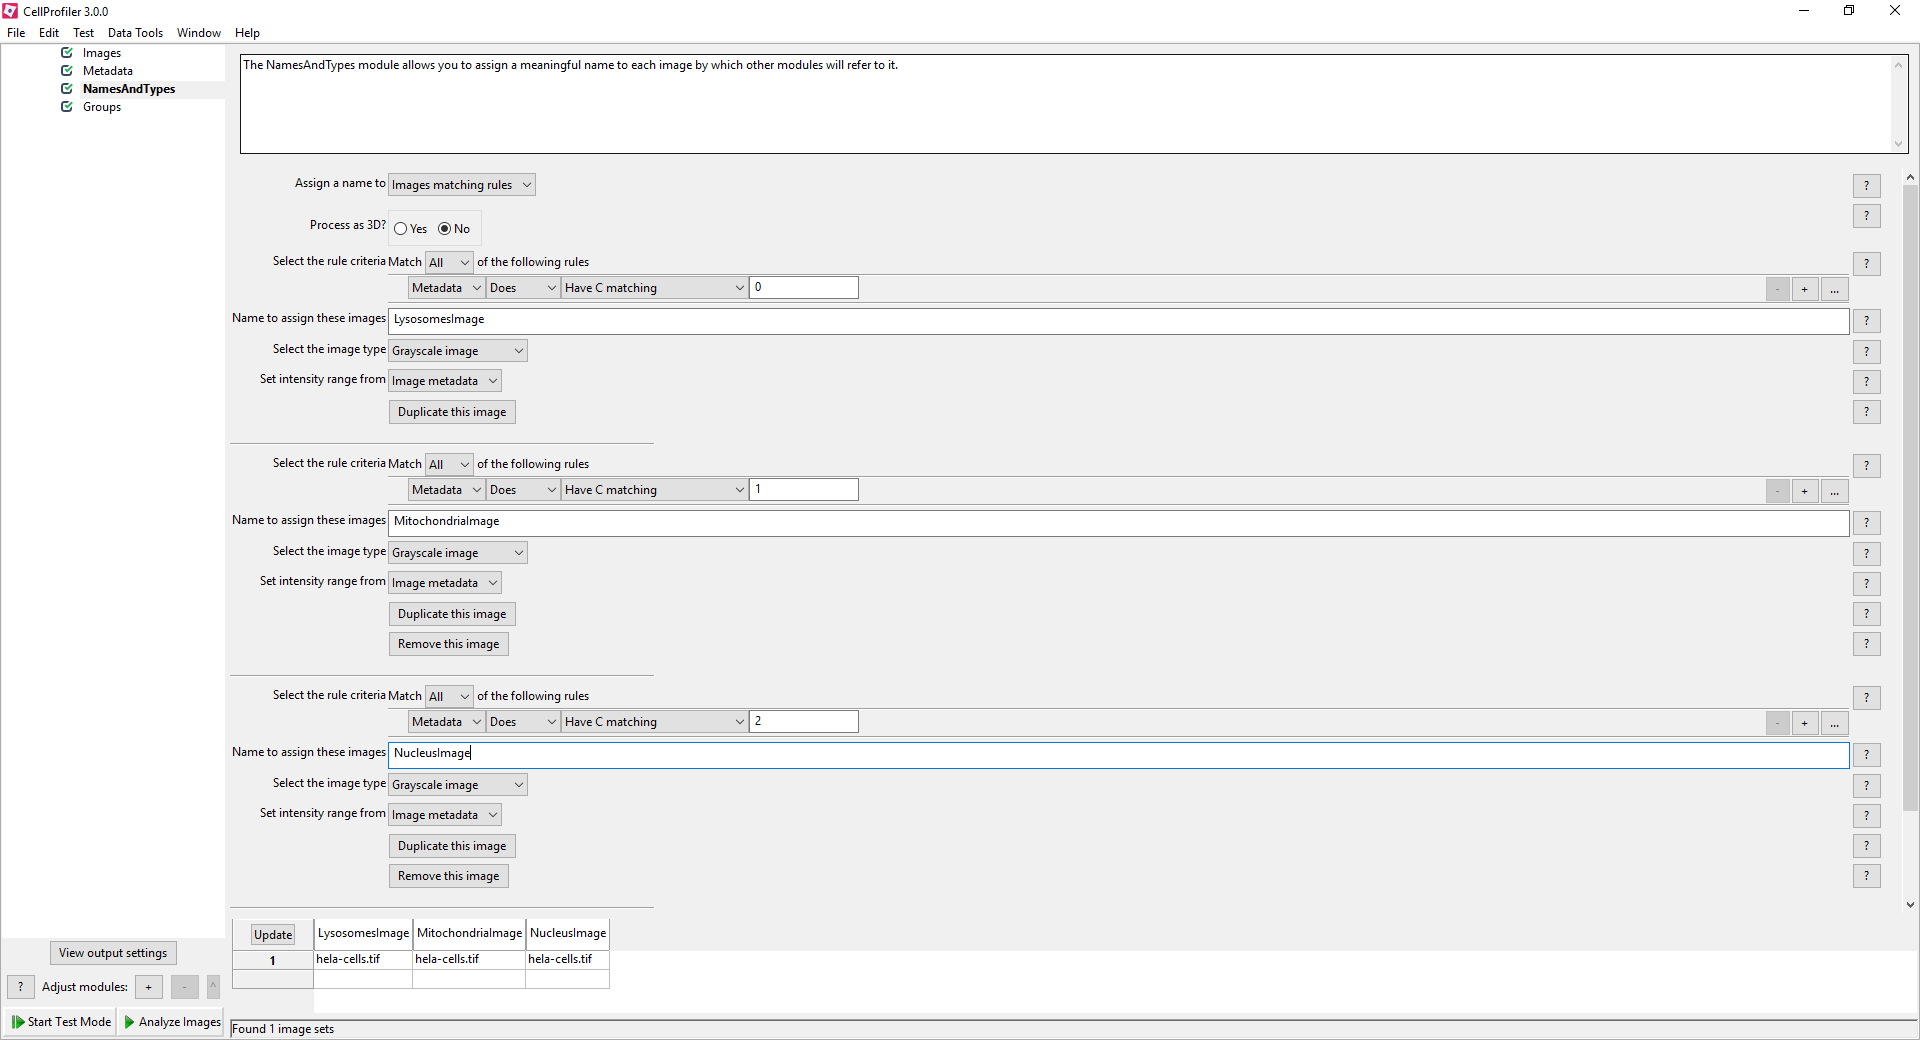
\includegraphics[width=0.70\textwidth]{mod4/figures/cpNamesAndTypes.png}
		  		}
		\medskip
		\captionof{figure}{Cellprofiler names and types module.}\label{fig:cpNamesAndTypes}
		\end{center}
	\end{minipage}
	
\item Make a \texttt{Right-Click} in the white area below the Group module. From the context menu select \texttt{[Object Processing > Identify Primary Objects]}.
Set \texttt{Select the input image}: \texttt{NucleusImage} and name the primary objects to be identified: \texttt{Nuclei}. Now
in the bottom left corner of the Cellprofiler window press \texttt{Start Test Mode} and the the \texttt{Run} button,
which appears immediately above.

A new window should pop up, which displays the original image and
further images with the outlines and colored areas of the detected nuclei as well as a result table. In the
outline image objects which were detected but do not meet the size criteria are outlined in mangenta
whereas accepted objects are outlined in green. The given set of parameters should have created an
oversegmented result. Estimate a realistic size range of the nuclei from the image (diameter in pixel
units!) and update the \texttt{Typical diameter of objects, in pixel units (Min, Max)} values in the
IdentifyPrimaryObjects module accordingly. Press \texttt{Run} again and check the results (You should obtain a
value of 4 for \# of accepted objects). Now go back to the IdentifyPrimaryObjects module and set \texttt{Use
advanced settings}: \texttt{Yes}. Play around with the options of \texttt{Threshold strategy} and \texttt{Thresholding method}.
Click on the \texttt{?}-buttons on the left, to learn more about the relevance of these options and
use the \texttt{Run} button to check the effect (cf. Fig. \ref{fig:cpIdentifyPrimary}).

	\begin{minipage}[t]{\linewidth}
		\begin{center}
		\adjustbox{valign=t}{%
		  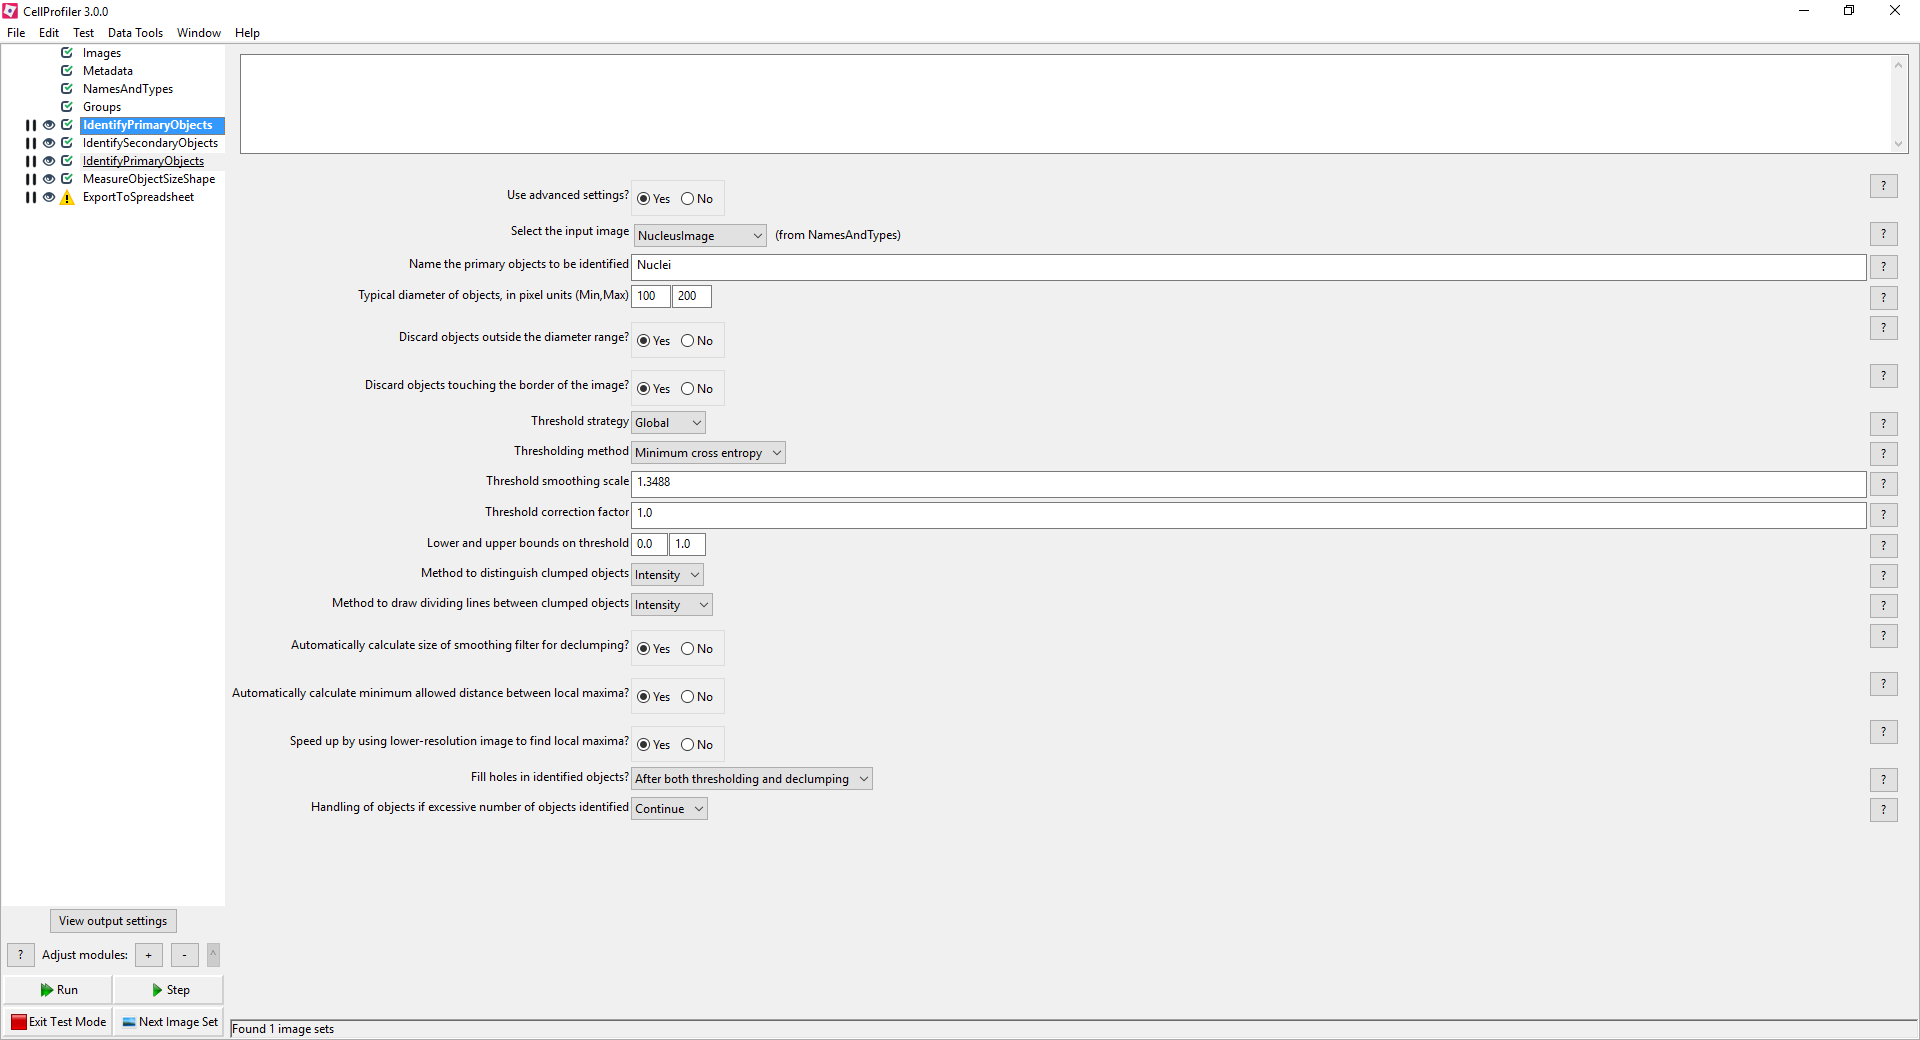
\includegraphics[width=0.70\textwidth]{mod4/figures/cpIdentifyPrimary.png}
		  		}
		\medskip
		\captionof{figure}{Cellprofiler identify primary objects module.}\label{fig:cpIdentifyPrimary}
		\end{center}
	\end{minipage}

\item Add another module \texttt{Right Click}, \texttt{[Add>Object Processing >IdentifySecondaryObjects]}. Set:\newline
\texttt{Select the input image}: \texttt{MitochondriaImage}\newline
\texttt{Select the input objects}: \texttt{Nuclei}\newline
\texttt{Name the objects to be}: \texttt{Cells}\newline
\texttt{Threshold correction factor}: \texttt{0.7}

Press the \texttt{Run} button again to check your results. Explore the additional settings in the
IdentifySecondaryObjects module and try to improve the segmentation (We want to segment the
complete cells here, not just the mitochondria) (cf. Fig. \ref{fig:cpIdentifySecondary}).

	\begin{minipage}[t]{\linewidth}
		\begin{center}
		\adjustbox{valign=t}{%
		  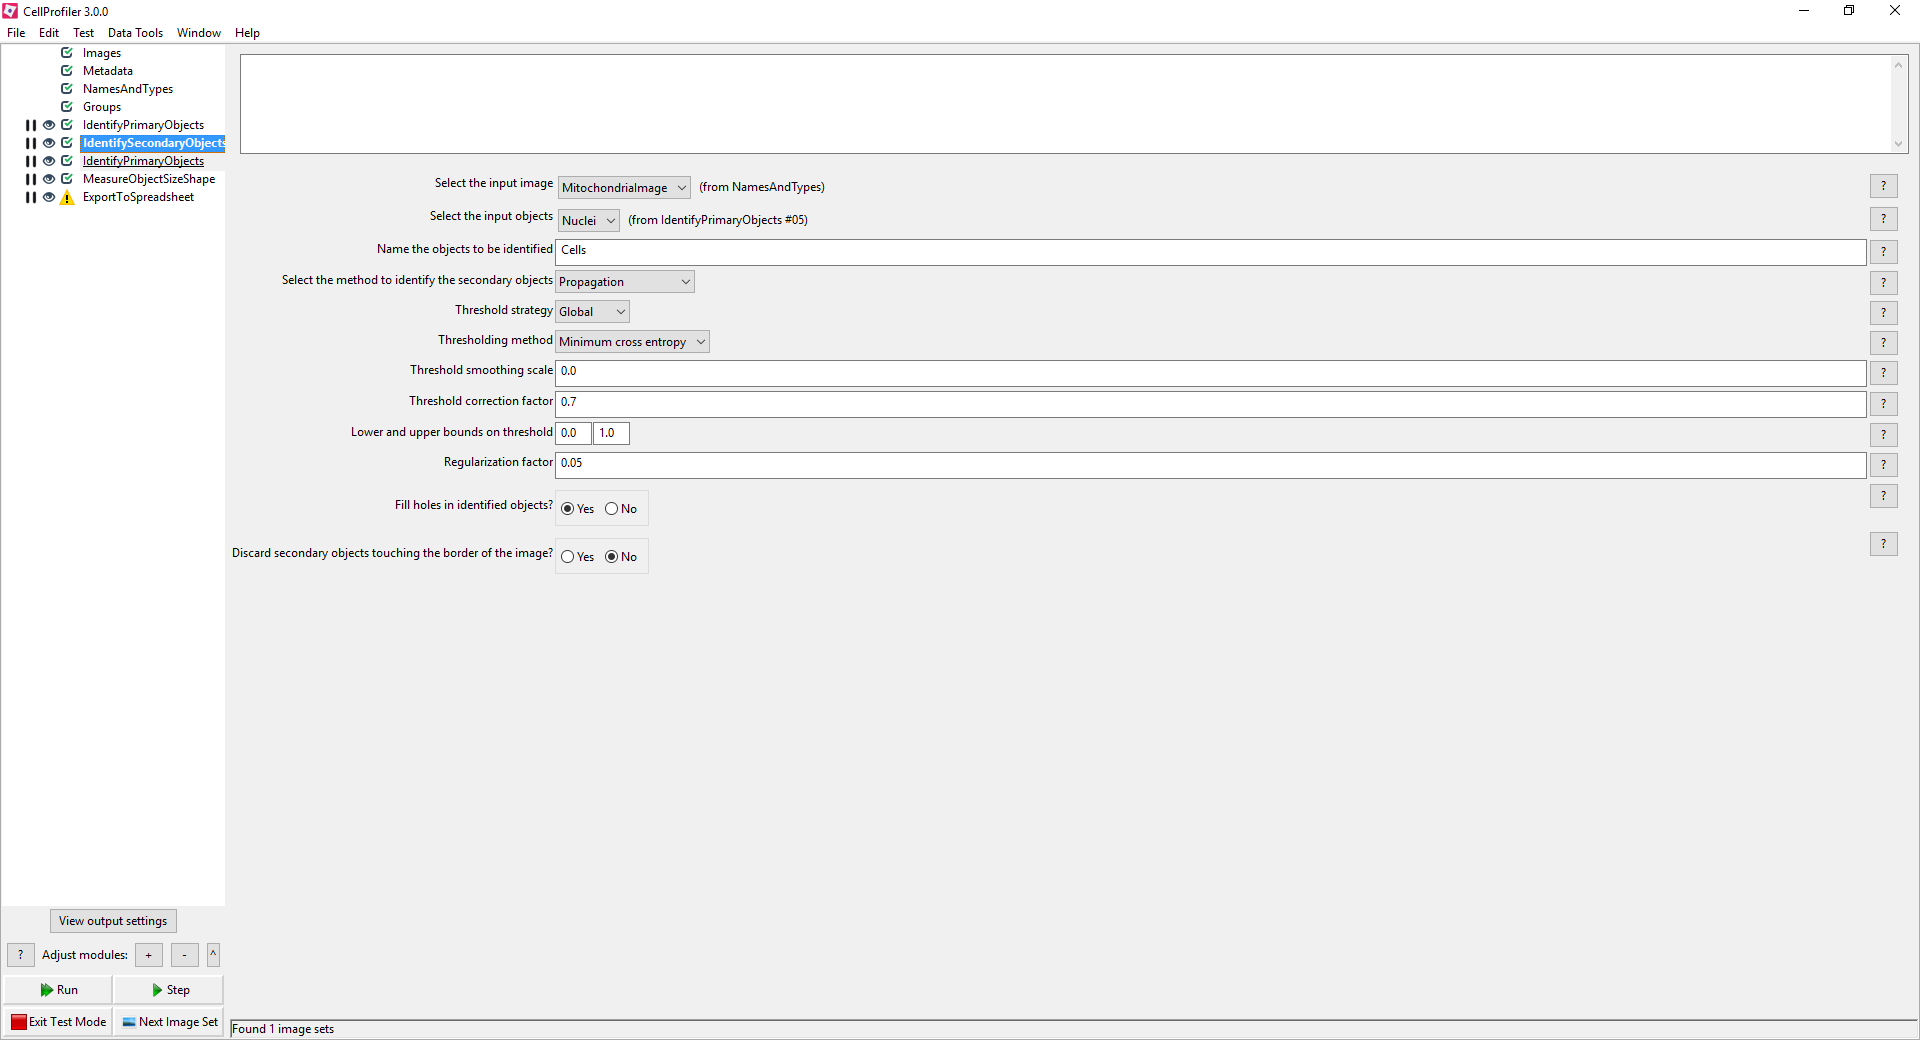
\includegraphics[width=0.70\textwidth]{mod4/figures/cpIdentifySecondary.png}
		  		}
		\medskip
		\captionof{figure}{Cellprofiler identify secondary objects module.}\label{fig:cpIdentifySecondary}
		\end{center}
	\end{minipage}

\item Add another module (\texttt{Right Click}, \texttt{[Add>Object Processing>IdentifyPrimaryObjects]}). Select the
LysosomesImage as input image and call the resulting objects lysosomes. Optimize the parameters for
optimal detection of lysosomes.

\item Now add another module \texttt{[Add>Measurement>MeasureObjectSizeAndShape]}. Select the \newline
\texttt{objects to measure}: \texttt{Lysosomes}. 

Set \texttt{Calculate the Zernike features?}: \texttt{No}. 

When you press \texttt{Run} the result window gives you the results aggregated per image. However, in the background a measurement for each
individual lysosome was performed. To obtain the detailed results we will export them to spreadsheet in
the next step.

\item Add another module \texttt{[Add>Data Tools>ExportToSpreadsheet]}. Change \newline 
\texttt{Output file location} to \texttt{Elsewhere…} and specify your Desktop folder below (cf. Fig. \ref{fig:cpExportSpreadsheet}).\newline 
Set \texttt{Select the measurements to export}: \texttt{Yes}.\newline
\texttt{Select measurements}: Expand the \texttt{Image} tree and check \texttt{Count}, expand \texttt{Lysosomes>Area and Shape} and
check \texttt{Area} and \texttt{MajorAxisLength}. \newline
Confirm with \texttt{OK}.\newline
Set \newline
\texttt{Calculate the per-image mean values for object measuremets?}: \texttt{Yes}.\newline
When you now hit the \texttt{Run} button a warning is displayed that spreadsheets will not be written out in test mode.
So we save our project \texttt{[File>Save Project]} and leave the test mode (Button \texttt{Exit Test Mode} in the lower
left corner). 
	\begin{minipage}[t]{\linewidth}
		\begin{center}
		\adjustbox{valign=t}{%
		  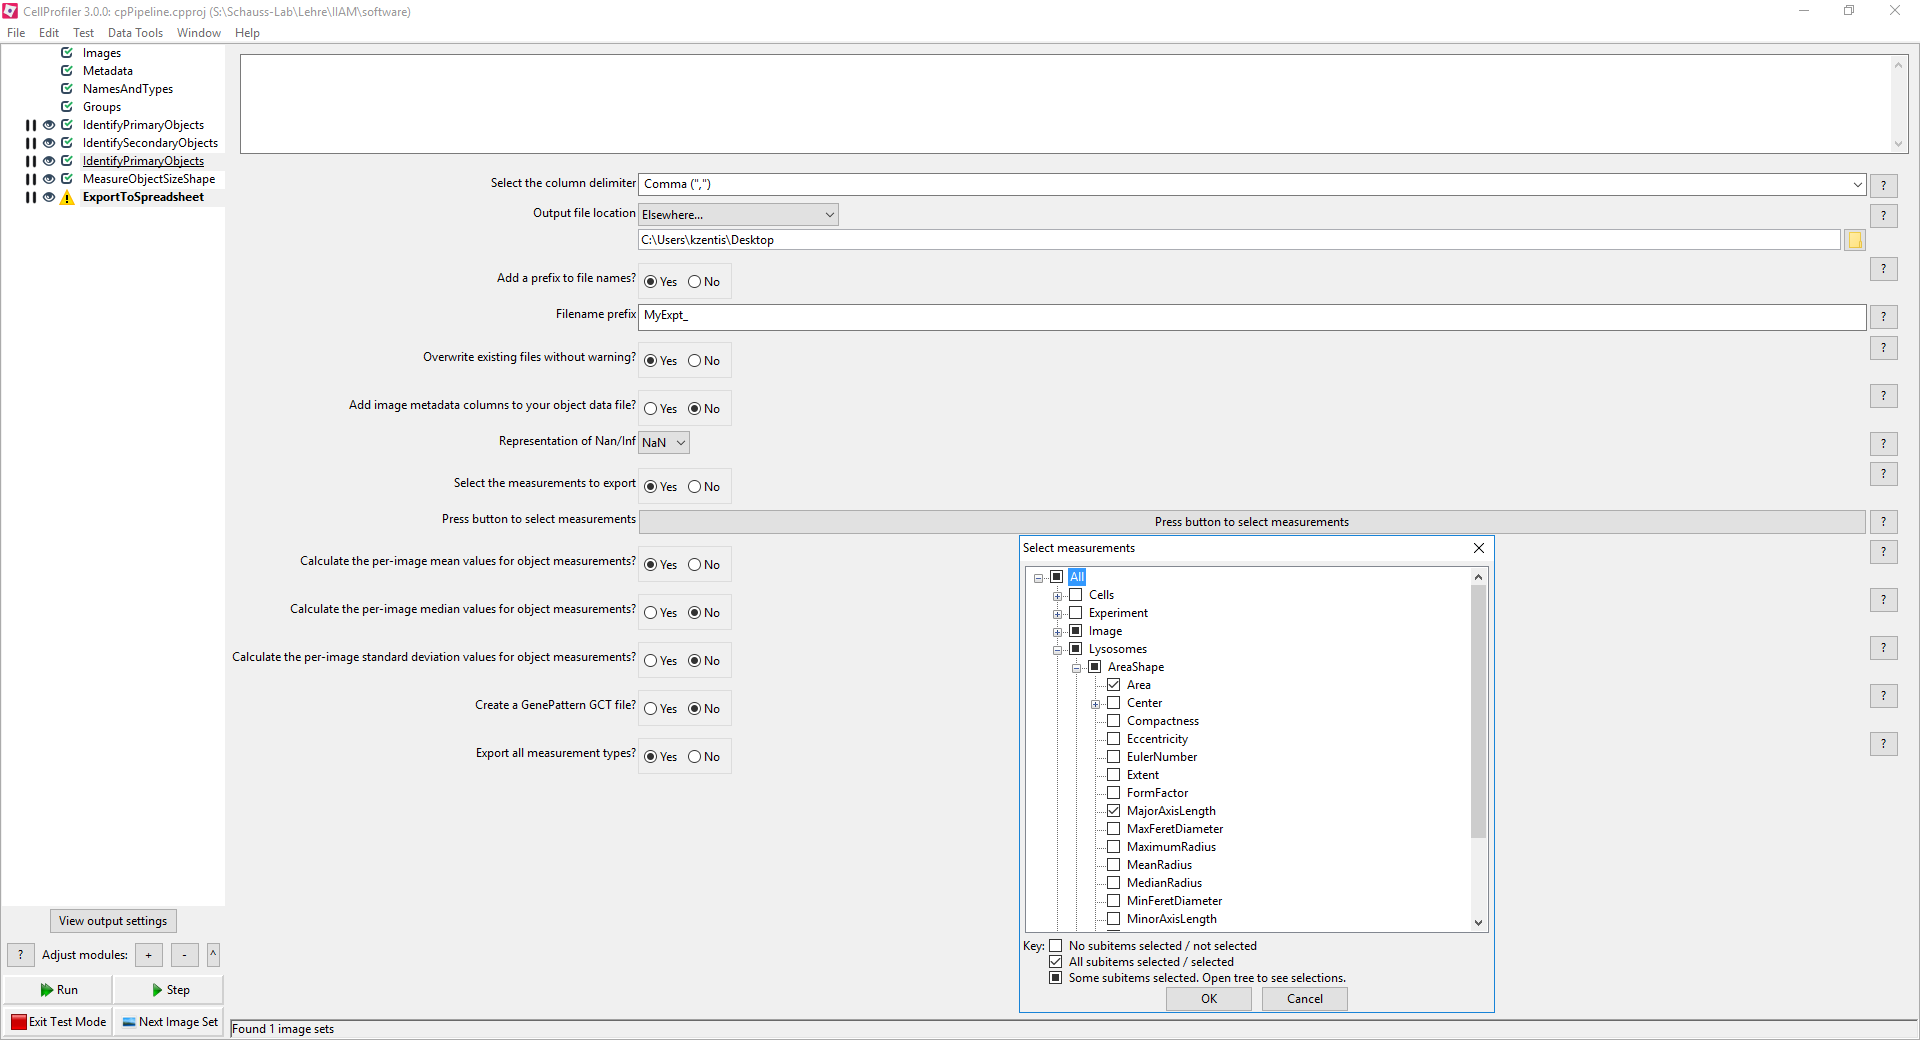
\includegraphics[width=0.70\textwidth]{mod4/figures/cpExportSpreadsheet.png}
		  		}
		\medskip
		\captionof{figure}{Cellprofiler export results to spreadsheet module.}\label{fig:cpExportSpreadsheet}
		\end{center}
	\end{minipage}

From the menu we select \texttt{[Window>Hide all windows on run]}. The little eye-icons left beside
the module in our pipeline should be grayed out now, which means they will not pop up the result
windows anymore. If you later on need to see them again just click on the according eye-icon. However,
during analysis it saves processing time not to display them. 

Now, start the analysis by clicking the \texttt{Analyze Images} button right beside the \texttt{Start Test Mode} button. After the analysis completed you will
find several csv-files on your Desktop. Use your favorite spreadsheet software to explore the contents - 
especially of the \texttt{image.csv}- and \texttt{lysosomes.csv}-file. \emph{Note that size measurements are expressed in pixel units, intensity as normalized intensity from 0 to 1.} Of course you can manually convert the results using
information from the metadata.

\item Two things are missing in our pipeline: The lysosomes are not yet assigned to a specific cell and we
might want to have some output images visualizing the results. So we go back to Cellprofiler. Add
another module \texttt{Add>Object Processing>RelateObjects}. Drag the module between the Identify Primary
Objects and the MeasureSizeAndShape module. Set \newline \texttt{Parent objects}: \texttt{Cell}/newline 
\texttt{Child objects}: \texttt{Lysosomes} \newline
and \texttt{calculate per-parent means for all child measurements?}: \texttt{Yes}.

Switch to the ExportToSpreadsheet module. In the \texttt{Select measurements} window additionally select
\texttt{Cells>Children>Lysosomes>Count and Lysosomes>Parent>Cells}. Repeat the analysis and check the
results. \emph{Note that the previous results will be overwritten!}

\item Add another module \texttt{Add>Image Processing>Overlay Outlines}. Set:\newline
\texttt{Select image on which to display outlines}: \texttt{LysosomesImage}\newline
\texttt{How to outline}: \texttt{Thick}\newline
\texttt{Select objects to display}: \texttt{Lysosomes}

Add another outline

Select \texttt{objects to display}: \texttt{Cells}\newline
	\begin{minipage}[t]{\linewidth}
		\begin{center}
		\adjustbox{valign=t}{%
		  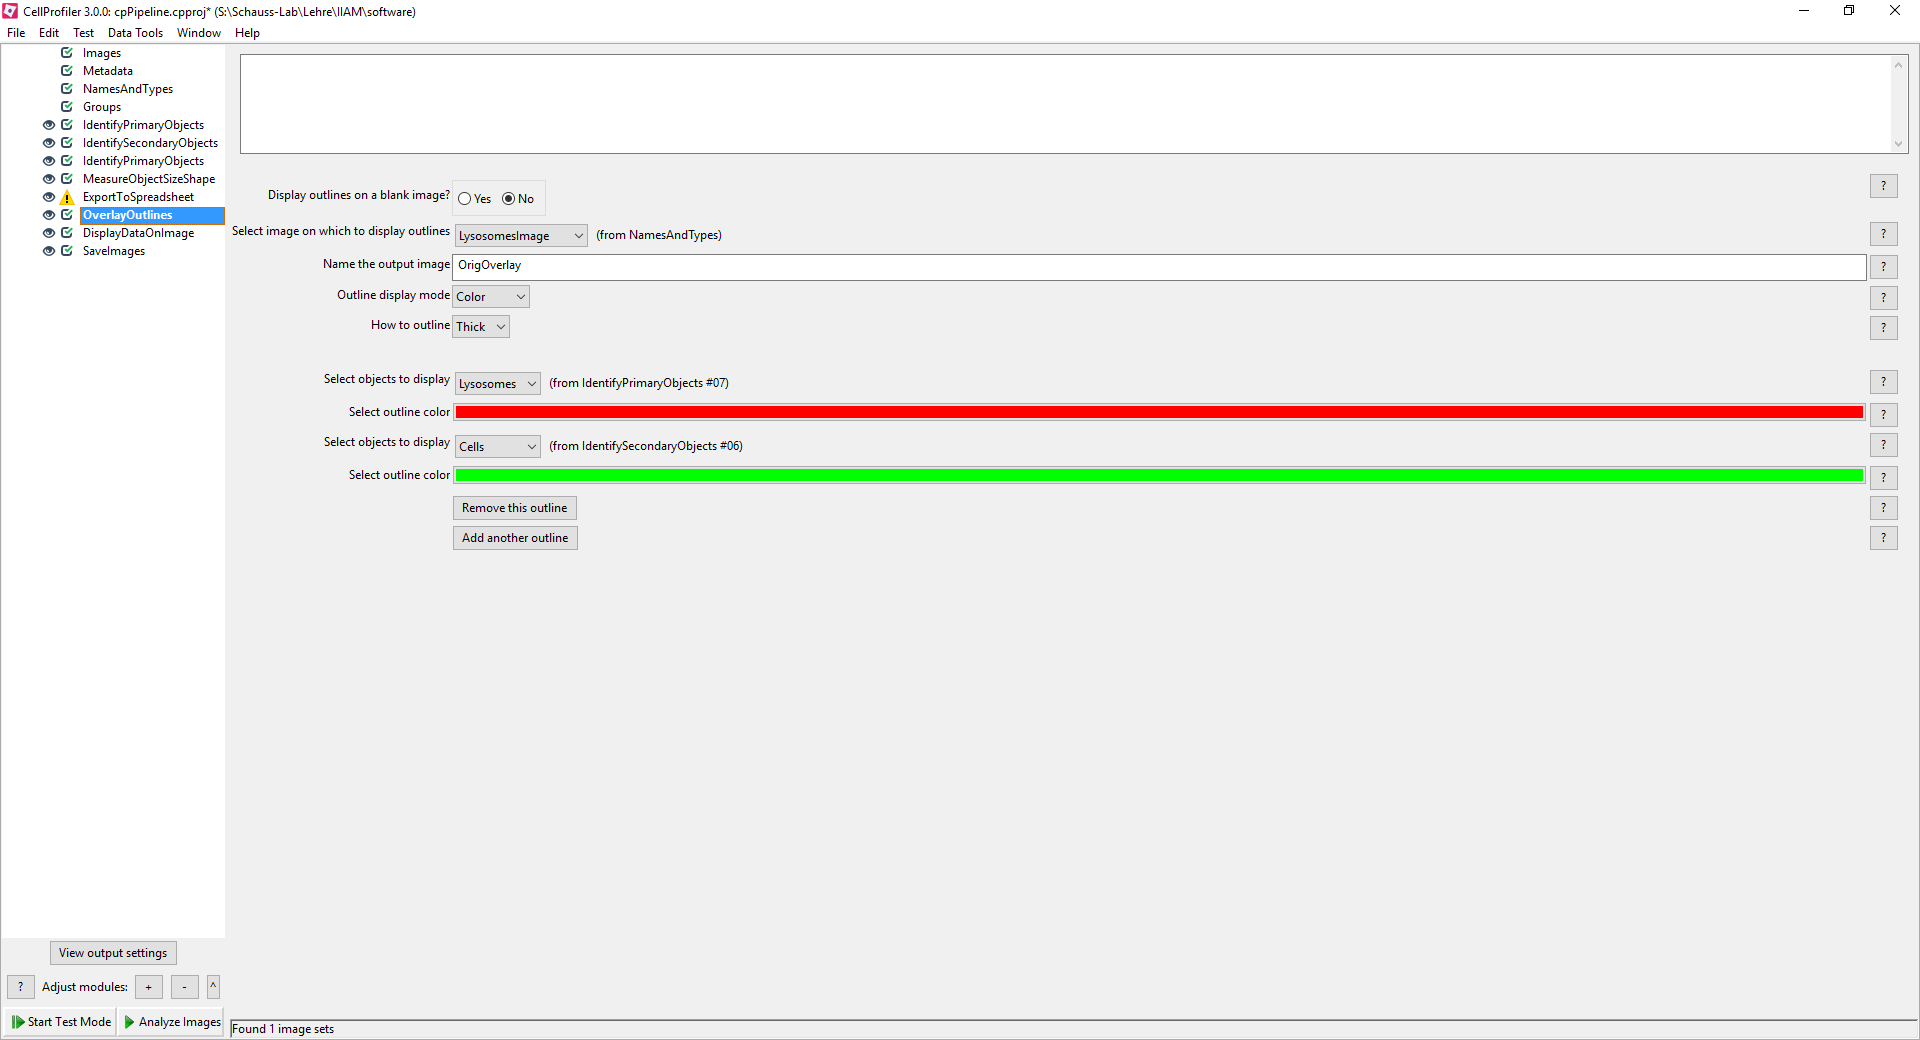
\includegraphics[width=0.70\textwidth]{mod4/figures/cpOverlayOutlines.png}
		  		}
		\medskip
		\captionof{figure}{Cellprofiler overlay outlines module.}\label{fig:cpOverlayOutlines}
		\end{center}
	\end{minipage}
	
\item Add another module \texttt{Add>Data Tools>DisplayDataOnImage}. Set:\newline
Select the \texttt{input objects}: \texttt{Lysosomes}\newline 
\texttt{Measurement to display Category}: \texttt{AreaShape}\newline 
\texttt{Measurement}: \texttt{Area}\newline
Select the \texttt{image on which to display the measurements}: \texttt{OrigOverlay}\newline 
	\begin{minipage}[t]{\linewidth}
		\begin{center}
		\adjustbox{valign=t}{%
		  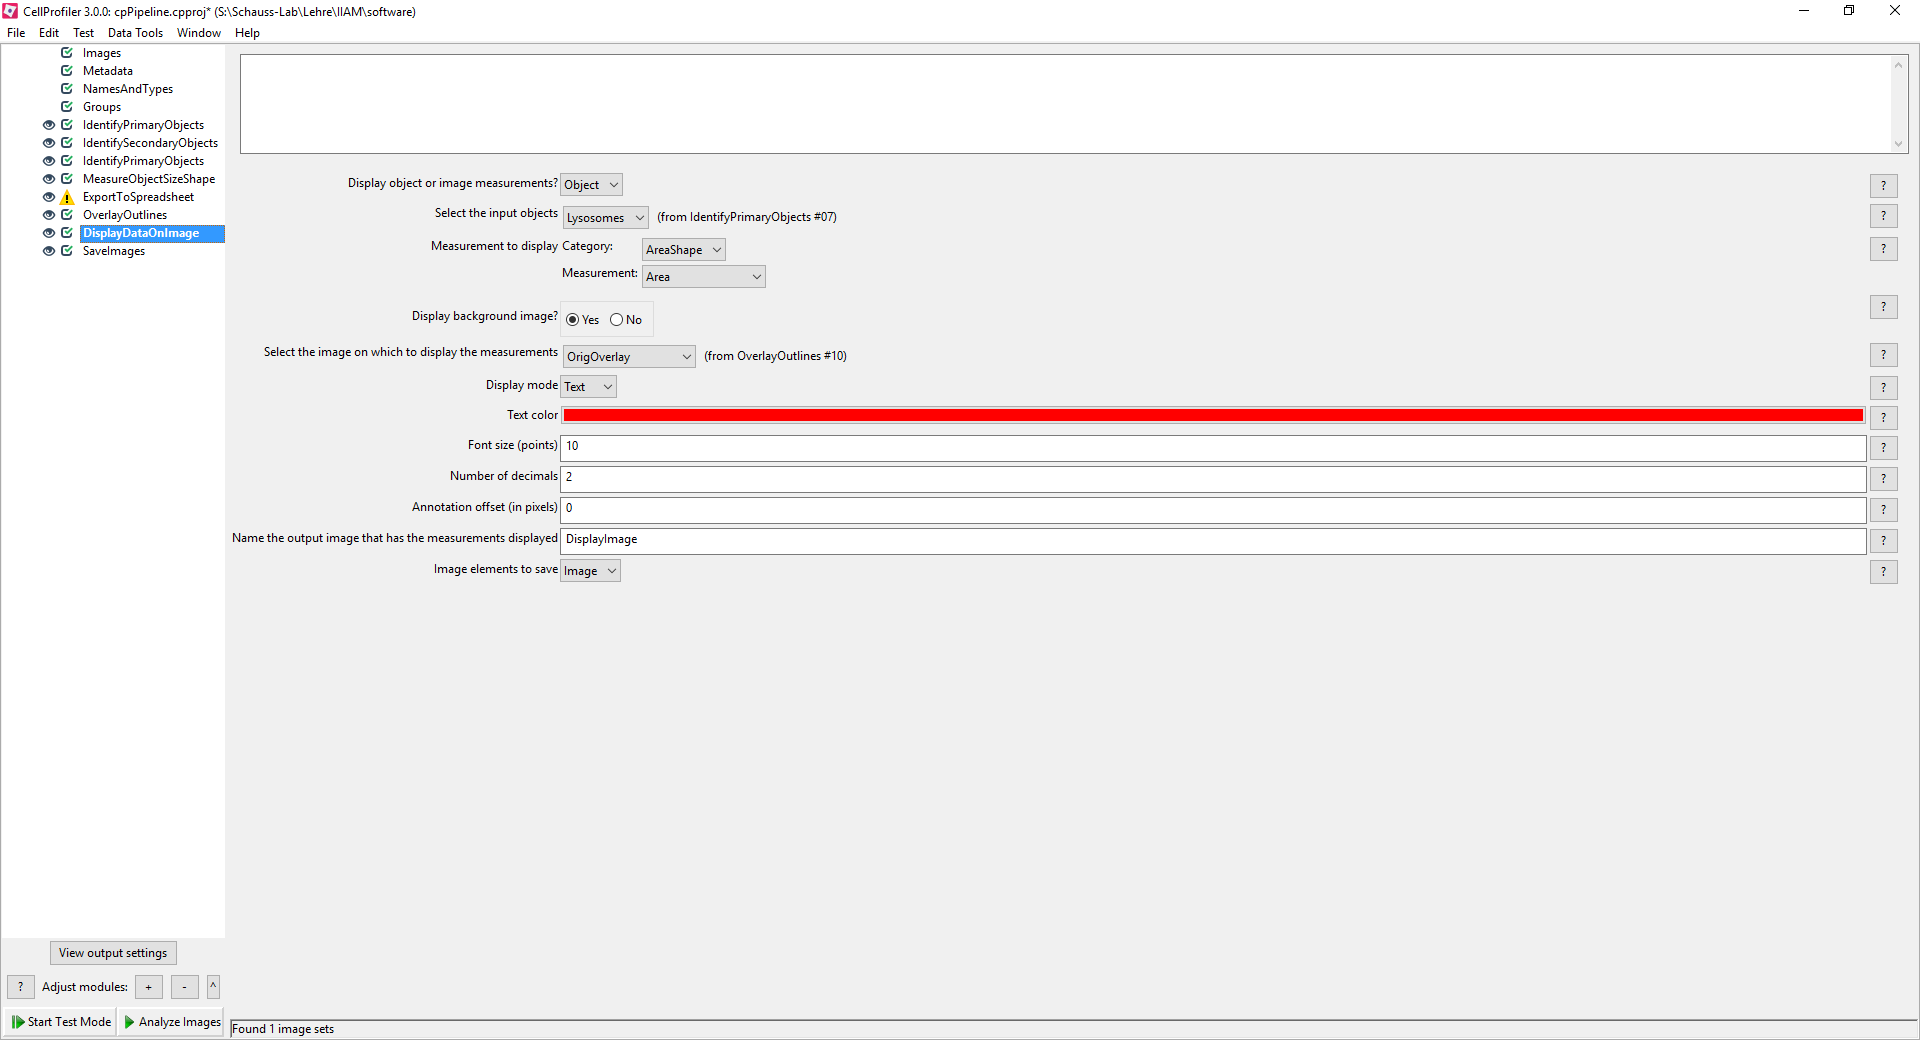
\includegraphics[width=0.70\textwidth]{mod4/figures/cpDisplayData.png}
		  		}
		\medskip
		\captionof{figure}{Cellprofiler display data on images module.}\label{fig:cpDisplayData}
		\end{center}
	\end{minipage}
	
\item Add another module \texttt{Add>File Processing> SaveImages}. Set:

Select the \texttt{image to save}: \texttt{DisplayImage}\newline
Select \texttt{image name for file prefix}: \texttt{LysosomeImage}\newline
\texttt{Saved file format}: \texttt{png}\newline
texttt{Output file location}: \texttt{Elsewhere…}\newline
\texttt{Subfolder}: Your Desktop.

	\begin{minipage}[t]{\linewidth}
		\begin{center}
		\adjustbox{valign=t}{%
		  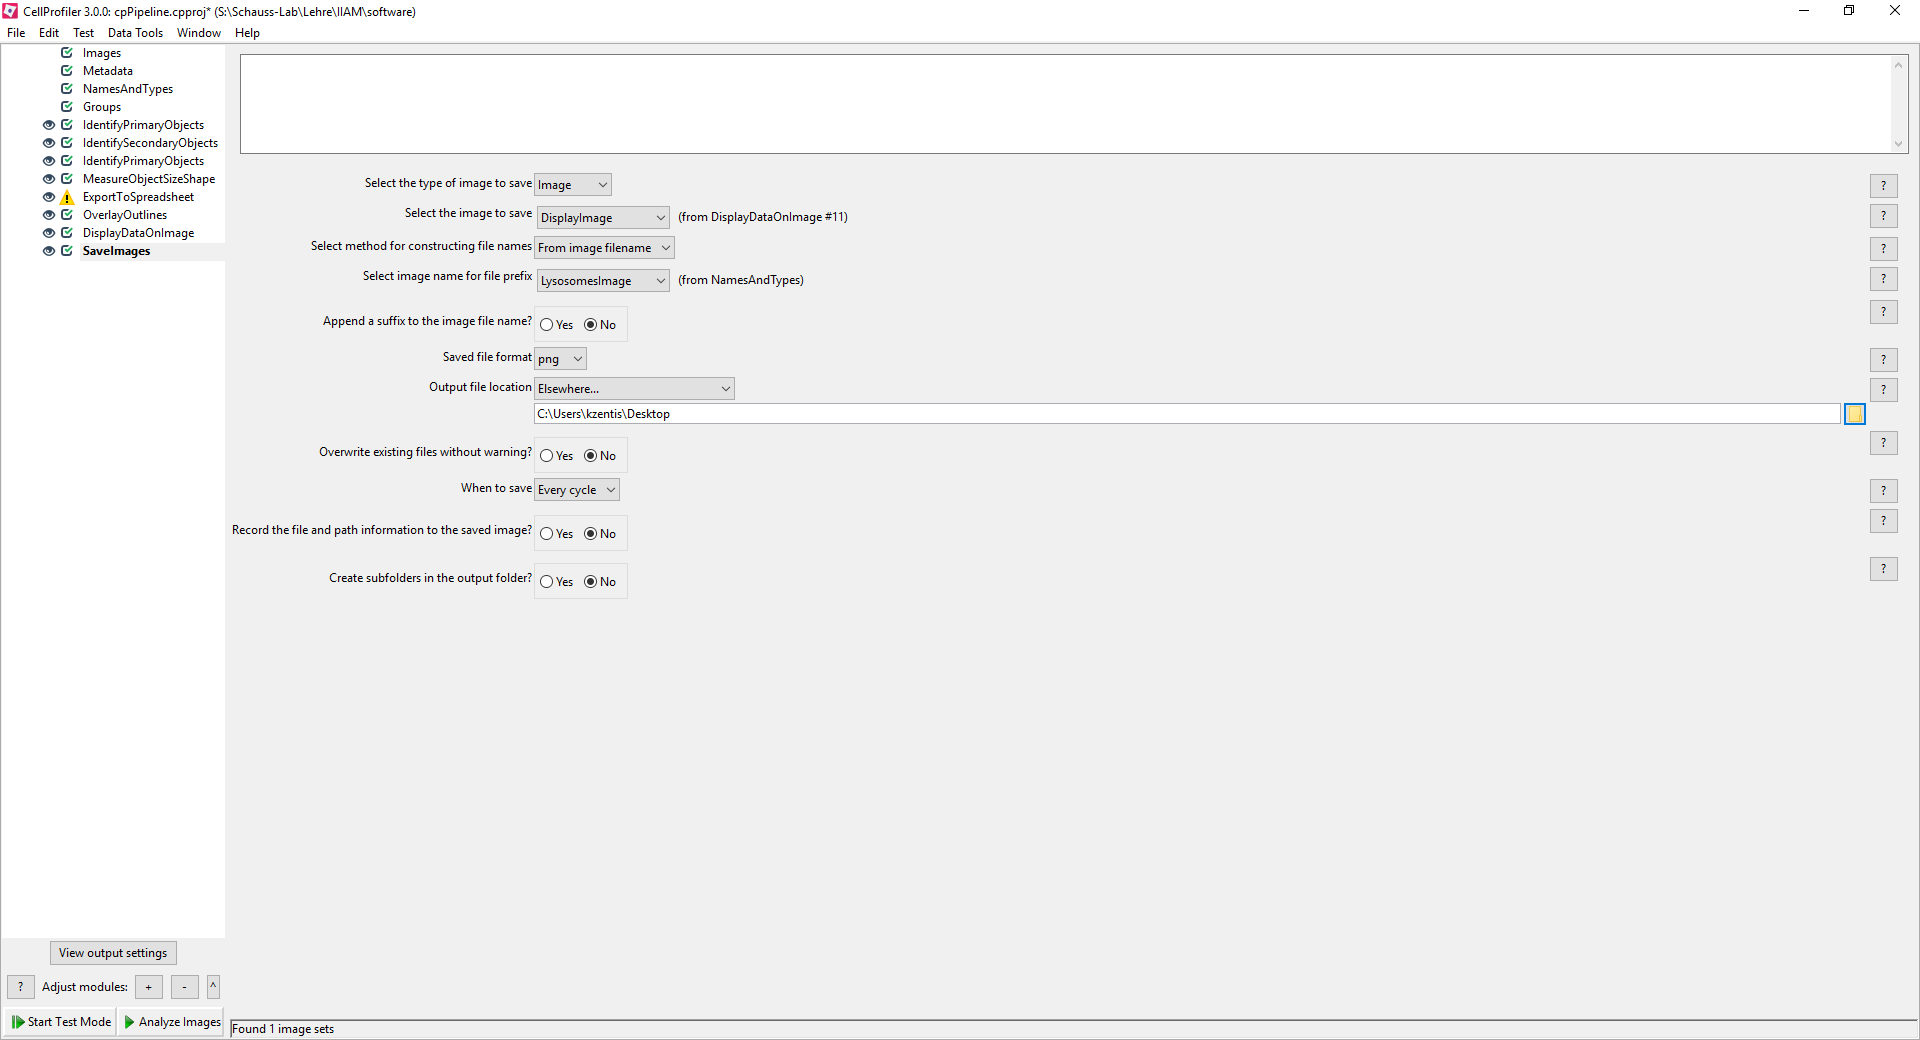
\includegraphics[width=0.70\textwidth]{mod4/figures/cpSaveImages.png}
		  		}
		\medskip
		\captionof{figure}{Cellprofiler save images module.}\label{fig:cpSaveImages}
		\end{center}
	\end{minipage}
	
When you run the analysis again, you should obtain an image with the outlines of cells and
lysosomes labeled with the measured size of the lysosomes.

\item Now we built a pipeline analyzing just one image. However, you could simply add further images to the
drop zone in the image pane and run the pipeline on all of them. Create a copy of the hela-cells.tif-file
with a different name and add it to the pipeline. Try to repeat
the analysis.

	
\end{enumerate}

\end{taskbox}









